\chapter{Discussion}
\label{Discussion}
The following chapter intends to discuss the results of the user study in correlation with comparing the results of the workshop and the card sort. Through this discussion it will be reflected upon how the findings leads to an understanding of the users' mental model.

\section{Comparing the results}
\label{ComparingResults}
As described in \autoref{ChapterWorkshop} is the scope of this user study to explore the users mental model of the TonePrint sharing platform. Which is an important aspect of designing the information architecture. In this pursue, two methods is used separately in order to explore how users group the concepts and functionalities of the platform and how they work together in order use the platform. In a perfect world could the results from this study indicate which content and concepts that should be present in different sites, in order to accommodate the users journey to complete a task. However isn't the world always perfect and the results might be to divers in order to be able to decide on a finished IA yet.

\subsection*{Comparing card sort and individual results}
\label{ComparingIndividualAndCard}
When looking at \autoref{UseOfCardSortData}, \autoref{IndividualTaskReflection} and \autoref{GroupTaskResults} is it very clear that the success of the two methods are very different. The results of the card is badly affected by the small sample size and lac of qualitative data, whereas the workshop provided a fair amount of data both from the individuals models which to some extend could be compared, and the discussion when agreeing on a model.\\
The scope of the individual task in the workshop was that the subjects had to find a TonePrint created by a fictional user. When comparing this task with the results of the card sort the starting point would be to look at the look at the groups focusing on "Finding TonePrints" and the cards representing the concepts and components, that the subjects uses in the workshop. Ass seen in
\autoref{IndividualTaskReflection} and the individual models \autoref{fig:ICMM1} to \autoref{fig:ICMM5} is the first step to either use a search function or filtering in a library or, in order to locate the corona toneprints created by 'User 1'. When looking at cards representing this such as \textit{TonePrint library}, \textit{Searching system} and \textit{'Effect type' filter} it's seen that they are located in the searching groups. For the aspect of filtering and searching on another user is the cards \textit{User library} and \textit{'User' filter} the best representatives whereas only the filter is seen as a searching tool. Bother of these is however grouped as a 'user feed' or 'User Profile', which is concepts that in some way also appears in the workshop results. There has not been provided cards that describes the use other users toneprints or in other ways is directly comparable with the aspects to which the 'User 1 profile' is used to find a 'User 1 corona TonePrint'. However does the two 'Profile', the 'User setting' and 'User feed' groups indicate that there should be some sort of user profile incorporated in the sharing platform. After locating the target TonePrint identifying it as a favorite is often the next step followed be downloading and beaming the TonePrint. While the \textit{TonePrint download system} and \textit{Beaming} cards are sorted in together identifying as a TonePrint software tools, the Favorite part is more difficult to compare, because no card or group is directly referring to the concept. The cards best most related to this is \textit{"Other users also liked this" recommendations}, \textit{'Rating' filter}, \textit{'Popularity' filter} and \textit{User raring system}. The first three of thees is always grouped together (When excluding subject 6) however is there little consistency in the groups thy are placed in, while the latter cards grouping have nothing in common that of the other. A comparison between the two methods for the part of favoring or rating a TonePrint to far-fetched.

\subsection*{Comparing card sort and group results}
\label{ComparingGroupAndCard}
The scope of the group task was to have the subjects finding an common ground for which concepts and functionalities that the sharing platform should feature. As seen in \autoref{GroupTaskResults} did this result in a description of a system whit somewhat well defined features. When looking at these results it's important to remember that the task dictated that when creating the TonePrint it should included a name, decription and tags used for categorizing the TonePrint. How they included and describes these is not hinted at.\\
When discussing the concept of tags and descriptions it's argued that they are very similar in the sense of describing the TonePrint, in order to make it easier to find. This is also the case of the \textit{TonePrint category}, \textit{Tags describing a TonePrint} and \textit{TonePrint description} cards which have been grouped together every time, belonging to groups either focused on searching or TonePrints in general. \textit{'Effect type' filter} and \textit{'Genre' filter} are cards that also is grouped for searching, which is quite similar to what is suggested in by the group, when suggesting what the tags might be based on.  As for the sharing aspect of the group discuss the two concepts, public and private. For the card sort is the cards \textit{Private forum} and \textit{Public forum} the most similar. These are almost pared by each subject and is grouped in 'Community' groups. This does not indicate that these cards might be related to the concept of sharing one's TonePrint. 

\subsection*{General comparison and reflection}
\label{CompareGeneral}
Despite the comparisons above is it still important to keep in mind that this data stems from a small number of people. This isn't as much a problem for the workshop, given the type of data, it is a larger problem for the card sort data. However, some tendencies is spotted where groups from the card sort, either by label or cards often paired together, draws similarities towards concepts or ideas generated though the workshop. This indicates that there might be some common ideas of how the concepts works for e.g filtering or tags and that there is some general idea of a profile being a part of the community. This is however just tendencies spotted in a small set of data hinting ad some similarities without statistical evidence. \\
The idea behind conducting the to studies simultaneously was to gather a large amount of data from the card sort, providing a clear indication of conceptual groups, which then would be compared to the conceptualized mental models from the workshop. It's always easy to be skeptical in retrospect when a study doesn't goes as planed. The card sort could have been conducted in person instead which would have made it possible to gather more qualitative data, but at the same time wouldn't it be able to reach user across the globe. A reason for conducting the card sort remote was also that it could "handle it self", allowing time to be allocated to the workshop and other aspects of the project.\\
When reflecting on the workshop there's also some perspective worth taking to consideration. The results derived from the individual tasks is based on five users ability to conceptualize and verbalize how they wants to solve a task, using an imaginary system. The number of participants of cause limits how much that might be derived from the workshop alone, however is it still possible to find tendencies with only few subject, when using qualitative methods. When subject conceptualize their mental model based on a task is the findings also limited to the extent of that task. An example from this study is that there seams to be a general idea of the concept of profiles. Because the task denotes that the subjects should locate a TonePrint is the only information derived for the profile that it contains the TonePrints created by that user. This doesn't mean that the users lack a mental model regarding what the profile concept might include, it just indicates that the their mental model of the profile concept tells them it can be used to access that users TonePrints. Instead of using the task focused approach could the subjects just have been told to "Name the concepts you think should be a part of the TonePritn sharing platform, and describe these concepts". By doing that is the task limitations avoided, however could this result in the subjects providing superficial descriptions because they lack a context to base it on. In order to reach the entire extend of the platform more studies should be conducted and even then would it be fare-fetch to state that the entire mental model has been explored, because the mental model. \\
Compared with the individual tasks the group task provides a more thorough description of the concepts used to complete the task, because the subjects are describing and discussing their understanding of the concept in order to reach a common consensus in the group. It could be argued that both tasks of the workshop should be conducted as group tasks, in order to get the a more thorough description of the concepts for the first task. However is it also possible that the group task went well because the subjects already ha framed their mindset towards creating concepts and verbalized them through the presentation, which means that each subject in the group task already was in a state of mind that may have affected the group discussion. If another workshop was to be conducted it should be considered to switch the task around, making the upload task individual and having it as the first and the task of finding a TonePrint last, as a group task.\\

\section{The mental model (for now)}
\label{MentalModelForNow}
The results derived from \autoref{CardSortAnalysis} and \autoref{WorkshopResults} have been compared and reflected upon in \autoref{ComparingResults} and now it's time to use that information. As described in \autoref{ChapterWorkshop} the aim of the user study is to explore the user mental model of the TonePrint community.\\ 
Through this study it's found that the TonePrint community should include a searching functionality which enables the user to find TonePrints by searching or filtering in a list by Effect type, name, Creator (Other users), parameters of the TonePrint described as tags and which ever tag ascribed to a TonePrint. There should be user profiles which is accessible though the search functionality. The Profile should include the TonePrints that user have defined as Public and maybe some personal remarks and description. The TonePrints should include descriptions that highlights the creators intentions with the TonePrint and maybe describing the settings of it. The TonePrint should also include tags that describes the parameters and effect type of the TonePrint, where some of them suggested to the creator based on the TonePrint parameters and description by the system, and some is created entirely by the creator. It should be possible to download the TonePrint to one's own unit and adding it to a favorite list. The TonePrints is either private and can't be accessed by others, it can be "unlisted" which only is accessible for users granted access or it can be public for every to access. A conceptualized model of the TonePrint based on the description above is presented at \autoref{fig:ConcludingModel}.\\
%
\begin{figure}[H]
	\centering
	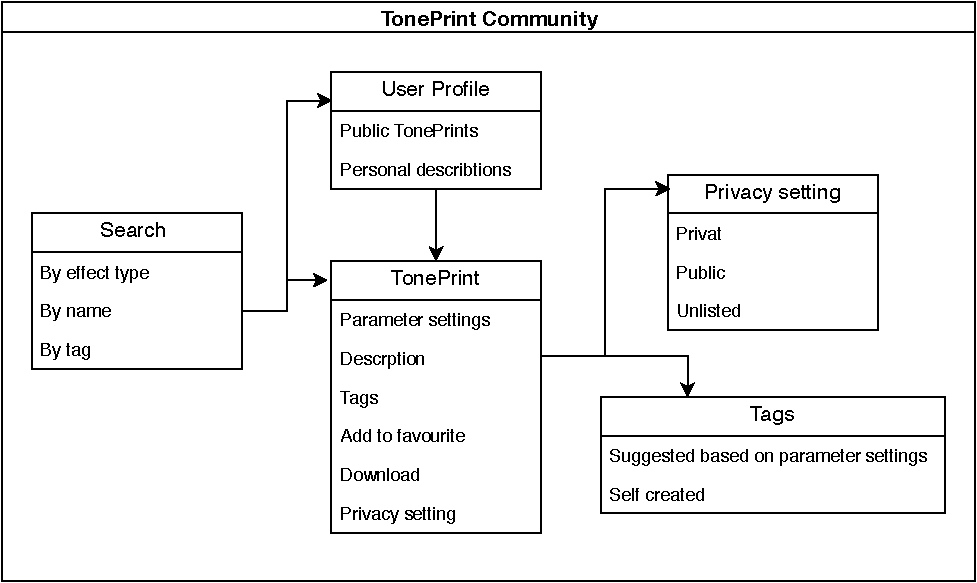
\includegraphics[width=0.7\textwidth]{ConcludingModel.pdf}
	\caption{The conceptualized Mental Model}
	\label{fig:ConcludingModel}
\end{figure}
%
\noindent
As made clear in \autoref{ComparingResults} does the mental model at \autoref{fig:ConcludingModel} not depict the entire community with all its concept and content, so to accommodate this new studies should be conducted focusing on both specif concept e.g how tags should be based on the parameters and how they are understood by the users, or specific groupings of content e.g what content should be on the same page and how should i be structured hierarchically. \\
Based on the findings of this study a new card sort could be conducted with with cards representing examples of content that belongs to the concepts seen on \autoref{fig:ConcludingModel}. This could be a closed card sort using the concepts as predefined groups. The results would then show to what extent the concepts are understandable. Another approach could be to create a Low-fidelity prototype based on this model, which than could be used to have the users conducting simple tasks exploring how the model derived from this study is interpreted by other users. Both approaches help exploring the understanding of the model in order to elaborate on it and create a design accommodating the mental model. 


